\documentclass[a4paper,12pt]{article} % добавить leqno в [] для нумерации слева
\usepackage[a4paper,top=1.3cm,bottom=2cm,left=1.5cm,right=1.5cm,marginparwidth=0.75cm]{geometry}
%%% Работа с русским языком
\usepackage{cmap}					% поиск в PDF
\usepackage{mathtext} 				% русские буквы в фомулах
\usepackage[T2A]{fontenc}			% кодировка
\usepackage[utf8]{inputenc}			% кодировка исходного текста
\usepackage[english,russian]{babel}	% локализация и переносы

\usepackage{graphicx}

\usepackage{wrapfig}
\usepackage{tabularx}

\usepackage{hyperref}
\usepackage[rgb]{xcolor}
\hypersetup{
colorlinks=true,urlcolor=blue
}
\usepackage{multirow}
\usepackage{hhline}


%%% Дополнительная работа с математикой
\usepackage{amsmath,amsfonts,amssymb,amsthm,mathtools} % AMS
\usepackage{icomma} % "Умная" запятая: $0,2$ --- число, $0, 2$ --- перечисление

%% Номера формул
\mathtoolsset{showonlyrefs=true} % Показывать номера только у тех формул, на которые есть \eqref{} в тексте.

%% Шрифты
\usepackage{euscript}	 % Шрифт Евклид
\usepackage{mathrsfs} % Красивый матшрифт

%% Свои команды
\DeclareMathOperator{\sgn}{\mathop{sgn}}

%% Перенос знаков в формулах (по Львовскому)
\newcommand*{\hm}[1]{#1\nobreak\discretionary{}
{\hbox{$\mathsurround=0pt #1$}}{}}

\begin{document}
	
	\begin{titlepage}
	\begin{center}
		{\large МОСКОВСКИЙ ФИЗИКО-ТЕХНИЧЕСКИЙ ИНСТИТУТ (НАЦИОНАЛЬНЫЙ ИССЛЕДОВАТЕЛЬСКИЙ УНИВЕРСИТЕТ)}
	\end{center}
	\begin{center}
		{\large Физтех-школа электроники, фотоники и молекулярной физики}
	\end{center}
	
	
	\vspace{4.5cm}
	{\huge
		\begin{center}
			{Лабораторная работа 6.11.2}\\
			Исследование фотопроводимости полупроводников
		\end{center}
	}
	\vspace{2cm}
	\begin{flushright}
		{\LARGE Салтыкова Дарья \\
			\vspace{0.5cm}
			Б04-105}
	\end{flushright}
	\vspace{8cm}
	\begin{center}
		Долгопрудный 2024
	\end{center}
\end{titlepage}

\noindent \textbf{Цель работы:} Исследовать собственную и примесную фотопроводимости. По полученной спектральной зависимости фототока определить ширину запрещенной зоны и энергию ионизации примеси полупроводника.

\section{Теоретические сведения}

Важной особенностью полупроводников является способность увеличивать электропроводность под действием света. Это явление получило название внутреннего фотоэффекта или фотопроводимости.

	Непосредственным результатом поглощения света в полупроводнике является увеличение числа свободных носителей тока. К поялению фотопроводимости приводят три типа переходов. В переходах первого типа электроны из заполненной зоны при поглозении фотона переводятся в хону проводимости. В результате этих переходов образуются свободные электроны и дырки. Возникающая при таких переходах фотопроводимости называется собственной. Переходы второго типа происходят при поглощении фотона атомом донорной примеси кристалла; при этом образуются свободные электроны и вакансии в донорных атомах. Переходы третьего типа возникают, когда при поглощении света электроны переходят из заполненной хоны на незанятые акцепторные уровни. В результате этого процесса образуются свободные дыки и электроны, связанные с акцепторными атомами. Фотопроводимость, возникающая в результате двух последних процессов, называется примесной.

	Некоторое количество носителей тока присутствует в полупроводниках и при отсутствии света. Часть электронов переходит их заполненной зоны (и с донорных уровней) в зону проводимости (и на акцепторные уровни) в результате теплового движения. Количество таких носителей -- и вместе с ним проводимость кристалла -- определяется температурой кристалла и быстро увеличивается при нагревании. В этом случае говорят о равновестных носителях тока и о темновой проводимости кристалла. Количество носителей тока равно равновесному не только в полной темноте, но и в тех случаях, когда энергия фотонов недостаточно велика для того, чтобы вызвать электронные переходы в кристалле. Фотопроводимость появляется лишь в том случае, если частота света выше пороговой. Эта мимнмальная частота, при которой начинается фотопроводимость, называется красной границей фотоэффекта.
	
	В отличие от тепловой, световая энергия запасается электронами полупроводника и практически не изменяет температуры кристаллической решетки. Поэтому в присутствии света тепловое равносвесие между электронами и решеткой нарушается. Носители тока, возникающие в результате оптической ионизации, являются неравновесными.

	После того как освещение кристалла прекращается, равновесие между электронами и решеткой восстанавливается. В обычных условиях энергия, запасенная неравновесными носителями тока, ничтожно мала по сравнению с тепловой энергией кристаллической решетки. Процесс установления теплового равновесия между решеткой и электронами сводится к тому, что неравновесны электроны и дырки рекомбинируют друг с другом, а температура кристалла практически не меняется. Не изменяется, следовательно, и концентрация равновесных носителей. Таким образом, можно считать, что включение и выключение света изменяет концентрацию неравновесных носителей и не влияет на концентрацию равновесных носитаелей тока.

	Измерение величины фототока может быть приведено по схеме, изображенной на рис. . Образец, изготовленный в виде пленки, включен в цепь, содержащую источник ЭДС и резистор, падение напряжения на котором измеряется цифровым вольтметром В7-34А. При освещении образца ток в цепи возрастает, возрастают и показания вольтметра. Подобного рода простые схемы пригодны для измерения только в том случае, когда фототок превосходит темновой ток или, в худшем случае, одного с ним порядка. Если это не так, приходится усложнять экспериментальную установку. Чаще всего при этом световой поток модулируется по амплитуде. Связанную со светом переменную составляющую полного тока нетрудно выделить на фоне даже очень большого постоянного по величине темнового тока.

	Зависимость величины фототока от частоты падающего света (спектральная зависимость фототока) имеет сложный вид, но ее характерной особенностью является наличие красной границы -- резкого обрыва кривой со стороны низких частот. Положение красной границы определяет наименьшую энергию фотонов, при которой может происходить образование носителей. Вид кривой вправо от красной границы (в сторону увеличения частот) может быть различным. После резкого подъема кривая фототока может быстро спадать (как у образца CdS), а может выходить на широкое плато (как например, у образца селена). Перед основным подъемом, соотвествующим энергии, при которой происходит переход электронов из заполненной зоны в зону проводимости, могут быть видны небольшие дополнительные максимумы. Эти максимумы связаны с примесными уровнями (переходы второго и третьего типа на рис. ). Как видно из рис. , энергия этих переходов меньше энергии, необходимой для перехода из заполненной зоны в зону проводимости, так что их красная граница находится слева от красной границы собственного перехода.

	Соотношение величины подъемов кривой фототока на собственных и на прмесных переходах зависит от концентрации примесей и от температуры. В чистых полупроводниках концентрация примесей очень мала. Кроме того, фотонное возбуждение примеси приводит к поялению всего одного носителя тока -- электрона или дырки, в то же время как при собсвенной проводимости полглощение каждого фотона сопровождается возникноваением электрона и дырки одновременно.

	С повышением температуры примесная фотопроводимость уменьшается быстрее, чем собственная. Может случиться, что уже при комнатной температуре большая часть примесных атомов термически ионизируется, и оставшаяся часть дает незначительный вклад в отопроводимость. Поэтому примесная фотопроводимость может оказаться значительно меньше собственной фотопроводимости.

	В предлагаемой работе положение примесных уровней и ширины запрещенной зоны полупроводника определяются по энергиям, при которых начинаются подъемы кривой фототока.

	Опыты проводятся на полупроводящих пленках или тонких пластинках монокристаллов CdS и CdSe с примесью ионов меди или без примеси. В отличие от большинства полупроводников, ширина запрещенной зоны у этих полупроводников сравнительно велика (более 1,5 эВ). Акцепторный уровень, обусловленный ионами меди, находится на большом удалении как от заполненной зоны, так и от зоны проводимости. В этих условиях красная граница примесной фотопроводимости лежит в области видимого света, в то время как у большинства других полупроводников она расположена в инфракрасной  области. Малый темновой ток и большой световой выход позволяют проводить опыты без модуляции светового потока.


\section{Экспериментальная установка}

Свет от источника И с помощью линзы Л фокусируется на входную щель монохроматора УМ-2. Эта щель находится в фокусе коллиматорной линзы $\text{Л}_1$.

	Параллельный пучок лучей, выходящий из линзы $\text{Л}_1$, разлагается в спектр призмой П. Выходная щель находится в фокальной плоскости окулярной линзы 2 и вырезает из спектра нужную область. Прошедший сквозь выходную щель свет падает на ячейку с исследуемым образцом, обозначенную на рисунке буквой Я. Последовательно с образцом включены стабилизированный выпрямитель, служащий источником ЭДС. Вольтметр В7-34А служит для измерения тока, протекающего через образец.

	\begin{figure}[ht!]
 	\center{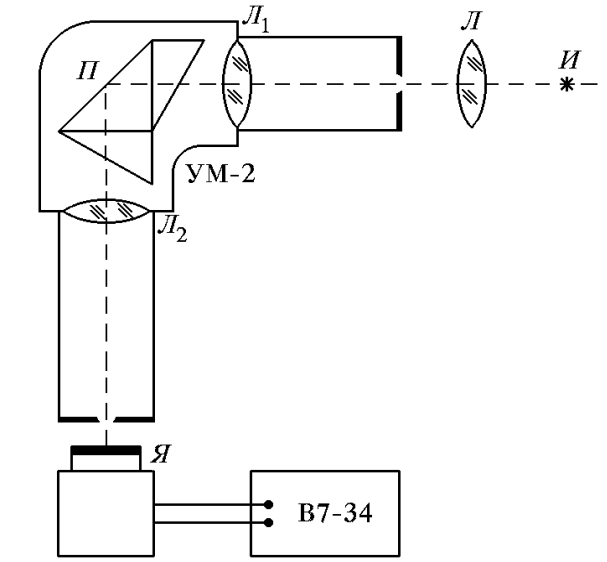
\includegraphics[width=0.4\linewidth]{scheme.PNG}}
	\caption{Схема установки для исследования спектральной зависимости фототока}
	\label{pic:scheme}
	\end{figure}
	
\section{Ход работы}
Проведем градуировку монохроматора. Проверку проведем по желтой линии неоновой лампы. Табличное значение $\lambda_{teor} = 5852\text{ \AA}$, на практике получаем 2513 дел., что соответствует $\lambda_{prak} = 5846\text{ \AA} .$ 

Снимем зависимость фототока от длины волны излучения. Напряжение измеряем на резисторе сопротивлением 40 кОм. Длину волны находим из калибровочного графика.

\subsection{CdSe}
Темновое напряжение образца 0,1 мВ.

Видим, что $СdSe$ имеет красную границу $\lambda = (8800 \pm 100)\text{ \AA}$. Получаем ширину запрещенной зоны, равную 1,41 эВ. При уменьшении длины волны кривая фототока выходит на плато. 

\begin{figure}[h!]
		\centering		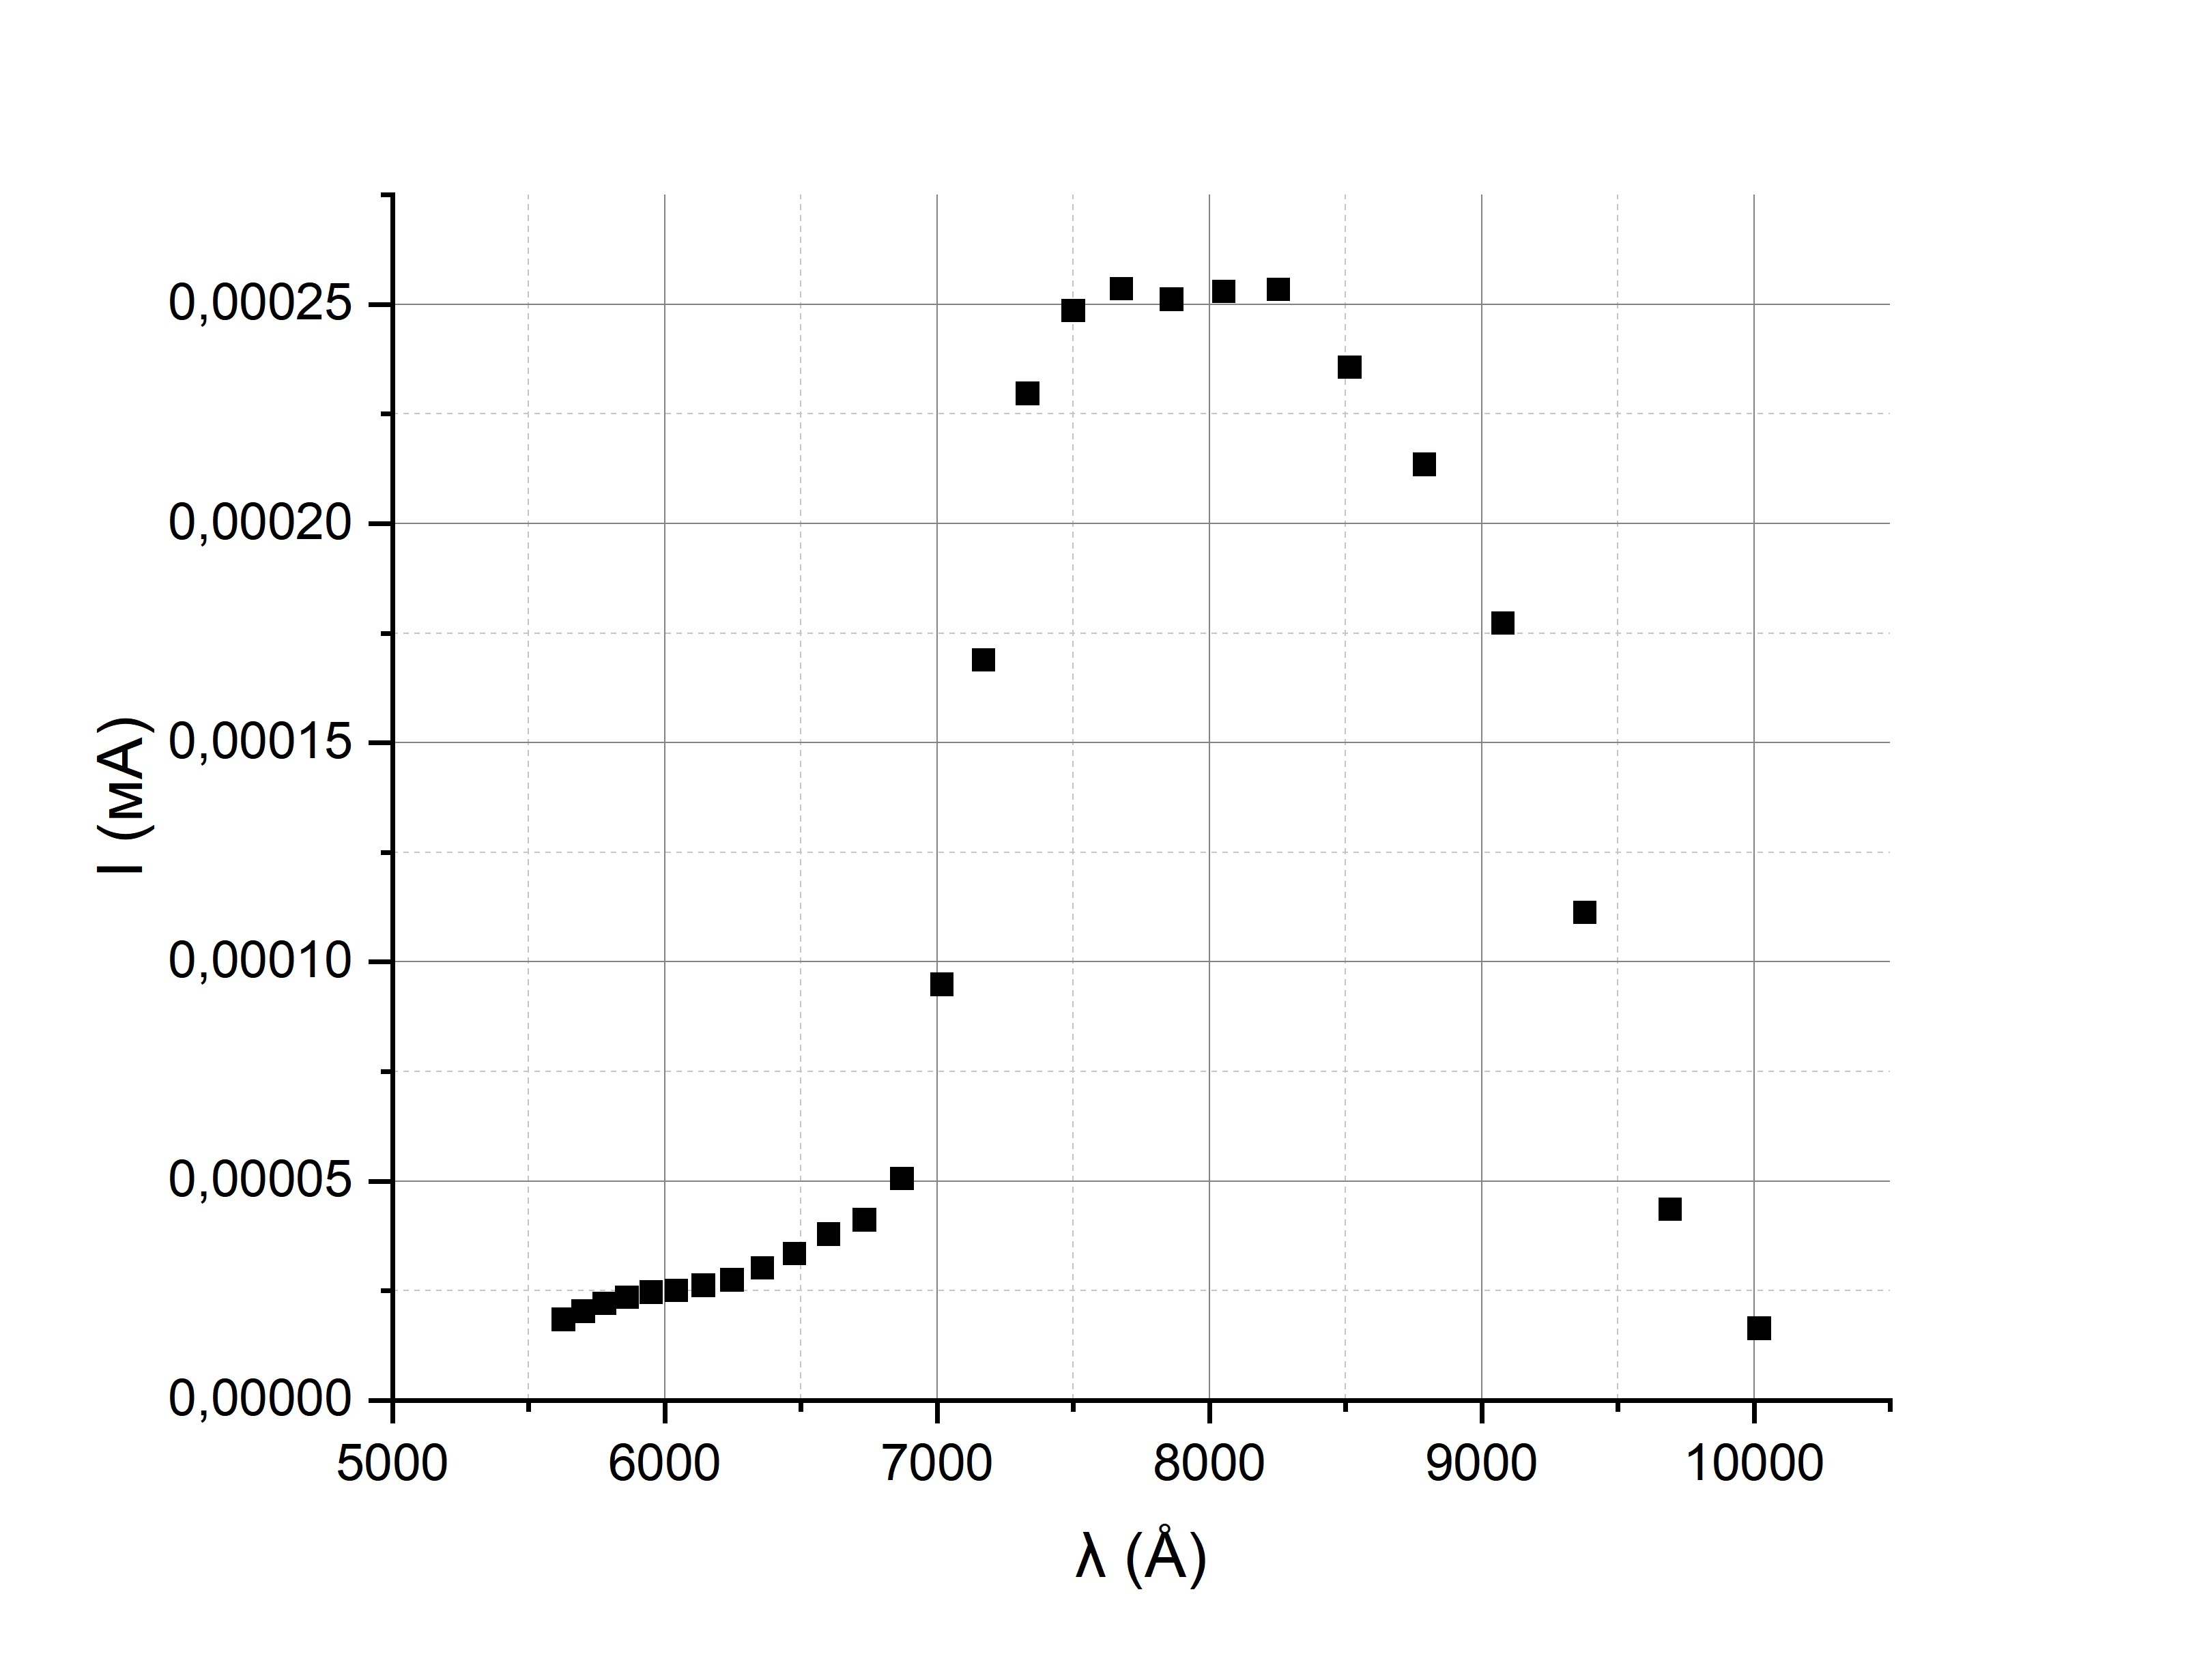
\includegraphics[width=0.7\textwidth]{CdSe.png}
		\caption{Cпектральная зависимость фототока от длины волны в образце CdSe}
		\label{pic:CdSe}
	\end{figure}
	

\subsection{CdS}
Темновое напряжение образца 1,5 мВ.

\begin{figure}[h!]
		\centering		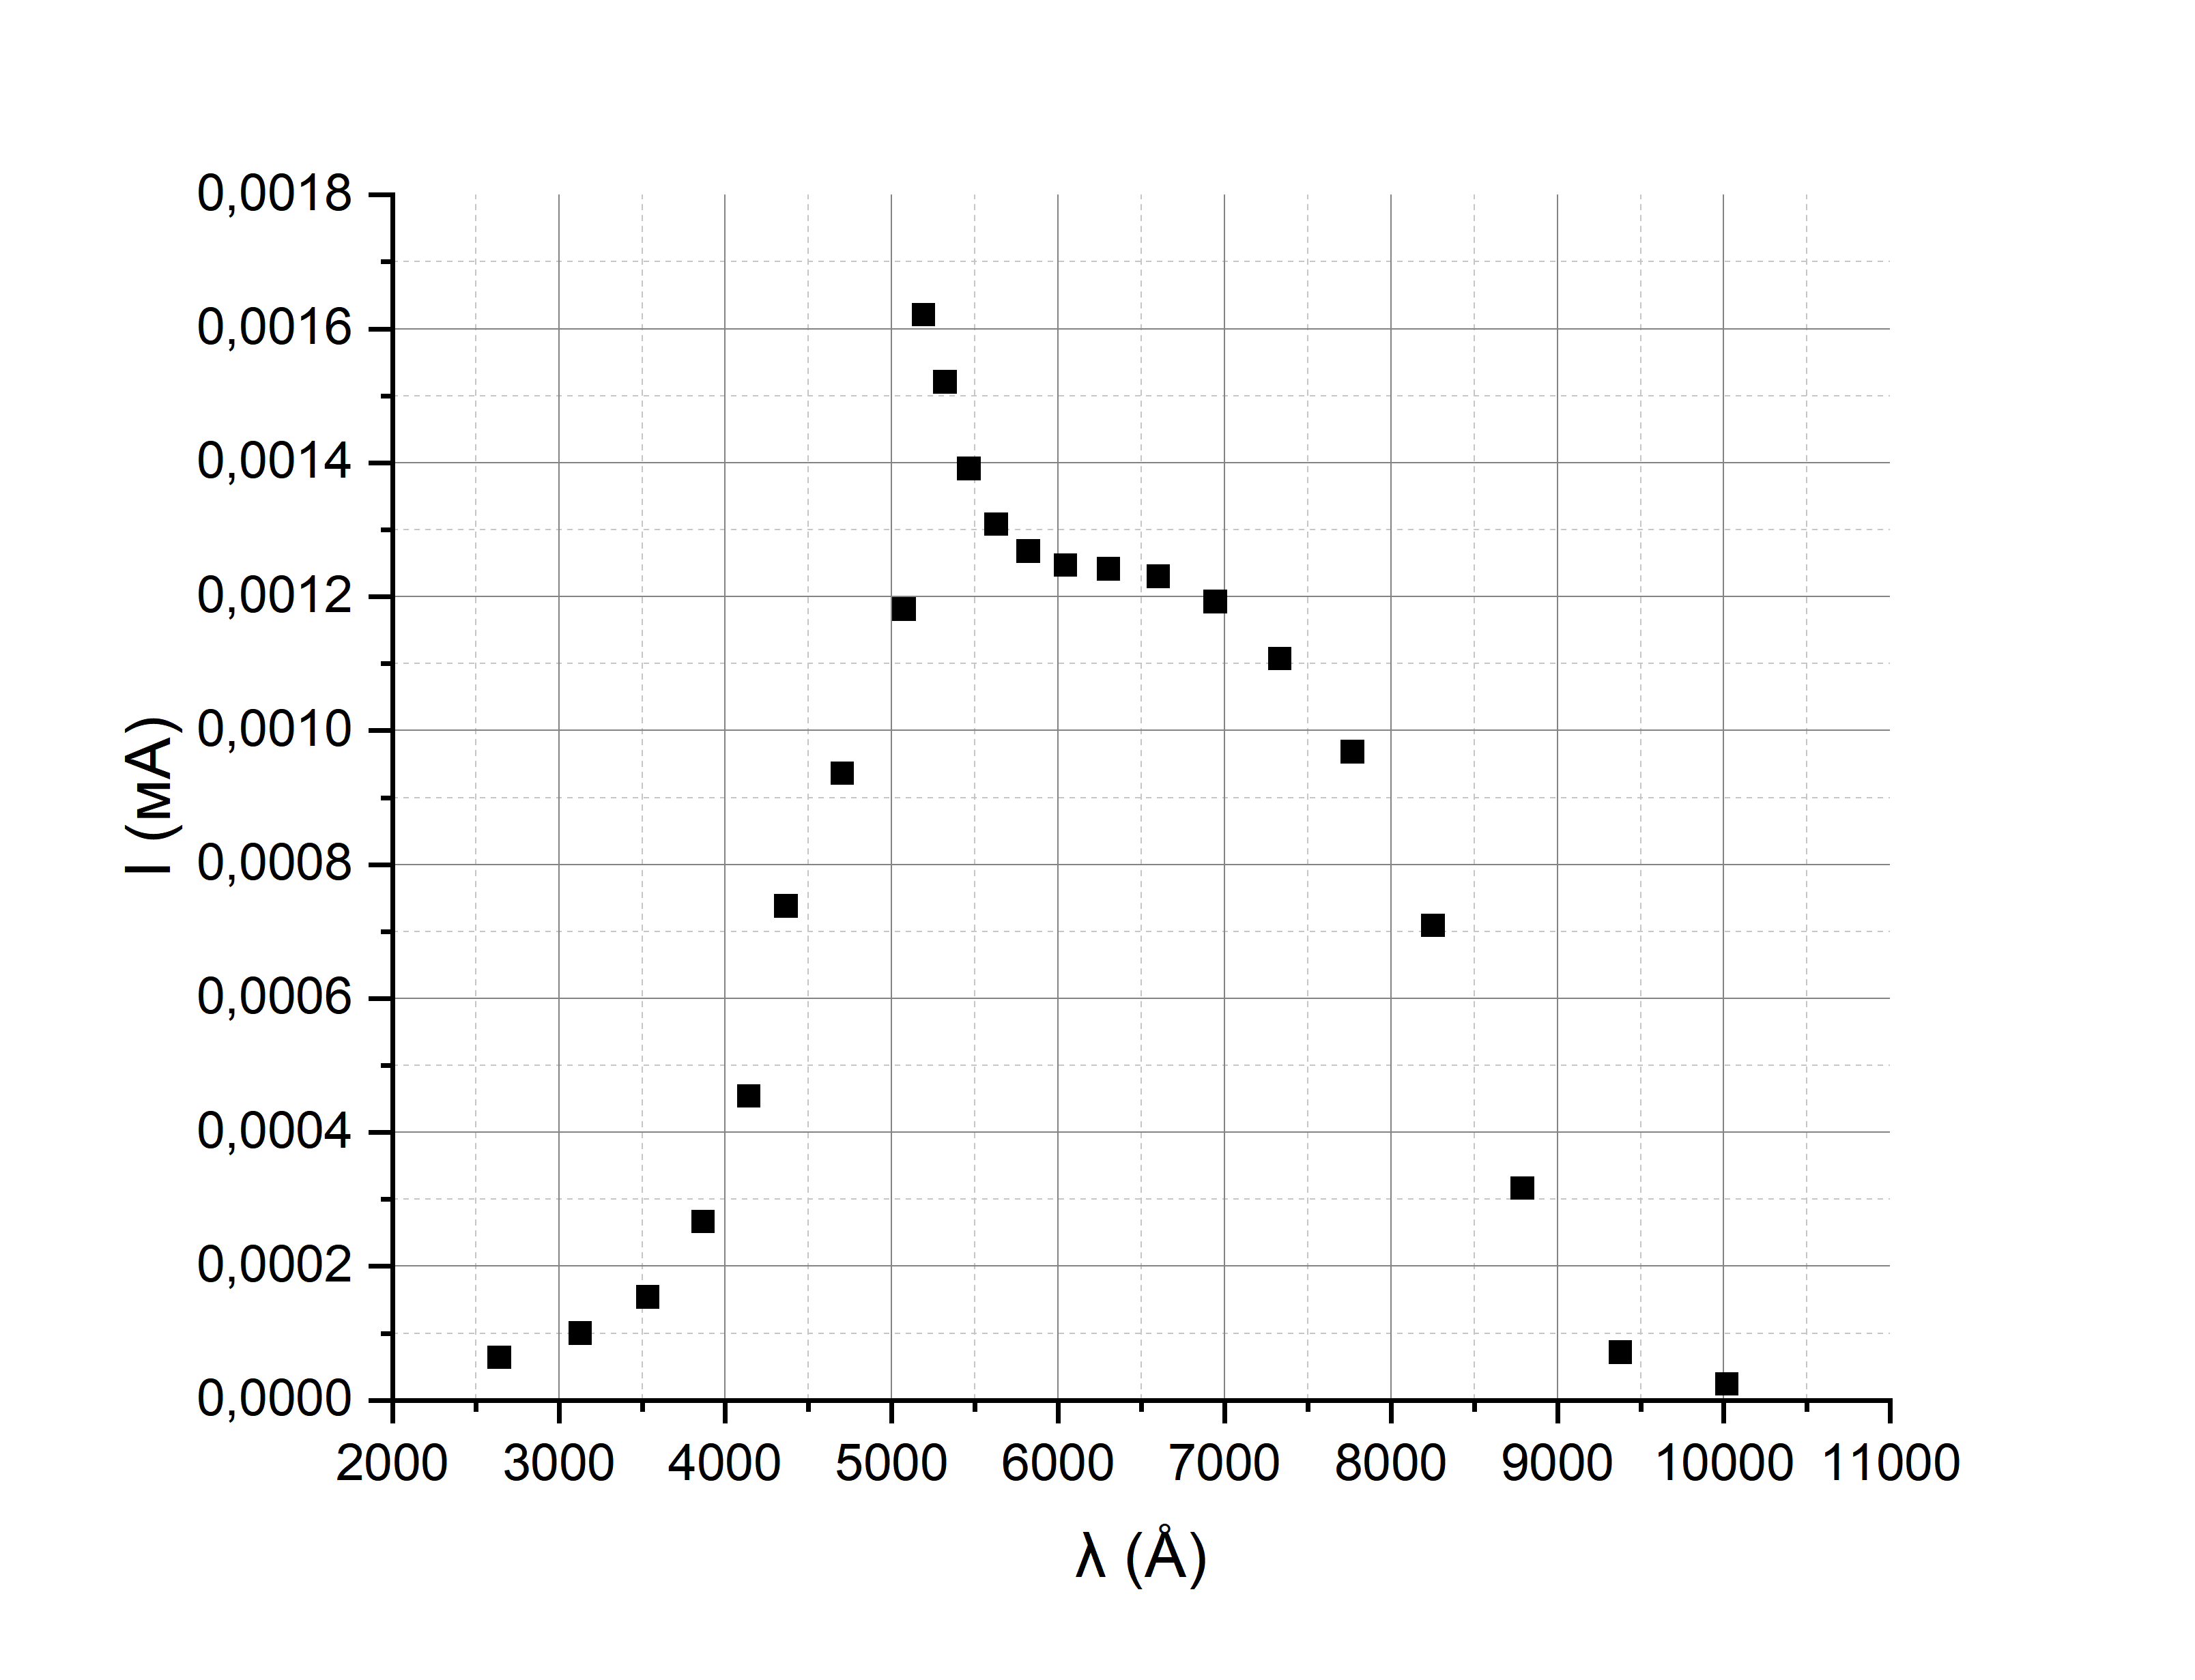
\includegraphics[width=0.7\textwidth]{CdS.png}
		\caption{Cпектральная зависимость фототока от длины волны в образце CdS}
		\label{pic:CdS}
	\end{figure}

Красная граница $\lambda = (5600 \pm 100)\text{ \AA}$. Ширина запрещенной зоны 2,21 эВ. На длине волны $7400\text{ \AA}$ (1,67 эВ) наблюдается подъем, связанный с примесными уровнями. 

\section{Вывод}
В ходе работы были исследованы спектральные зависимости фототока для двух образцов: CdSe и CdS. Полученные значения красных границ и ширин запрещенных зон, а также их табличные значения, приведены в таблице:

\begin{table}[h!]
\begin{tabular}{|l|l|l|l|}
\hline
Образец & $\lambda_{\text{кр}}, \text{ \AA} $ & $\Delta,$ эВ & $\Delta^{\text{табл}}$, эВ \\ \hline
CdSe    & 8800                                & 1,41         & 1,74                       \\ \hline
CdS     & 5600                                & 2,21         & 2,42                       \\ \hline
\end{tabular}
\end{table}



\end{document}